\documentclass{standalone}
\usepackage{pgfplots}
\pgfplotsset{compat=newest}

\begin{document}
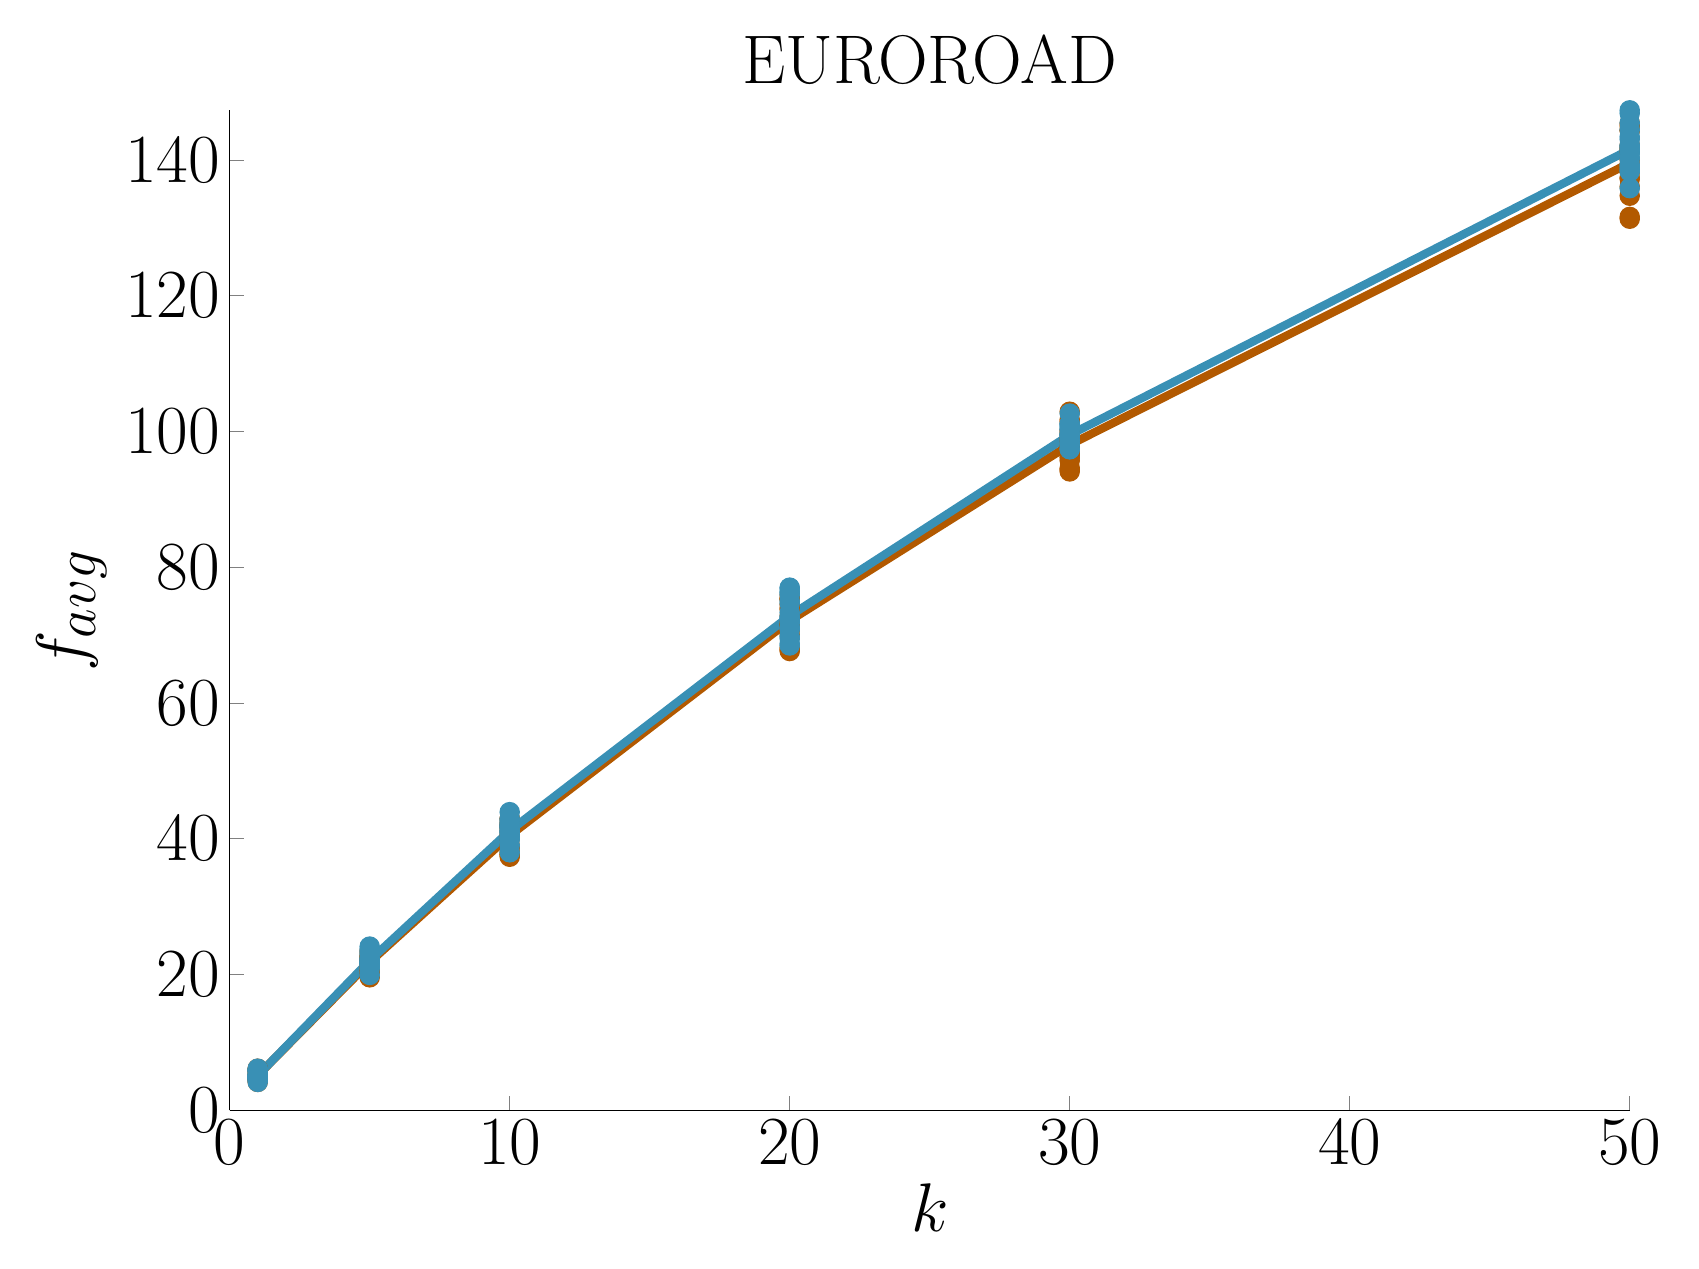
\begin{tikzpicture}

\begin{axis}[%
title style={font=\Huge},
title=EUROROAD,
tick label style={font=\Huge},
label style={font=\Huge},
legend style={font=\Huge},
view={0}{90},
max space between ticks=50pt,
width=7in,
height=5in,
scale only axis,
xmin=0, xmax=50,
xtick={0, 10, 20, 30, 40, 50},
xlabel={$k$},
ymin=0, ymax=147.3,
%ytick={0, 200, 400, 600, 800, 1000},
ylabel={$f_{avg}$},
major tick length=5pt,
axis lines*=left,
legend cell align=left,
clip=false]

\addplot [
only marks,
mark=*,
mark size=3.5pt,
color=orange!70!black,
%solid,
%line width=2pt,
]
coordinates{
(1,4.18)(1,4.44)(1,4.66)(1,4.71)(1,4.73)(1,4.77)(1,4.92)(1,4.97)(1,5.0)(1,5.03)(1,5.04)(1,5.04)(1,5.14)(1,5.16)(1,5.2)(1,5.68)(1,5.8)(1,5.89)(1,5.95)(1,6.13)(5,19.59)(5,20.19)(5,20.61)(5,20.97)(5,21.03)(5,21.28)(5,21.5)(5,21.56)(5,21.75)(5,21.79)(5,22.0)(5,22.03)(5,22.31)(5,22.39)(5,22.4)(5,22.54)(5,22.73)(5,22.83)(5,23.24)(5,23.5)(10,37.35)(10,37.67)(10,37.67)(10,38.06)(10,38.7)(10,39.0)(10,40.13)(10,40.19)(10,40.38)(10,40.49)(10,40.88)(10,41.13)(10,41.56)(10,41.62)(10,41.96)(10,41.97)(10,42.14)(10,42.4)(10,42.91)(10,42.94)(20,67.65)(20,67.82)(20,68.11)(20,70.03)(20,70.77)(20,70.92)(20,71.26)(20,71.67)(20,71.69)(20,71.78)(20,71.79)(20,71.79)(20,72.85)(20,73.81)(20,73.98)(20,74.52)(20,75.27)(20,75.32)(20,75.39)(20,75.91)(30,94.11)(30,94.4)(30,94.58)(30,95.71)(30,96.14)(30,96.48)(30,96.81)(30,96.83)(30,97.57)(30,97.79)(30,98.38)(30,98.43)(30,98.82)(30,98.85)(30,99.54)(30,99.9)(30,100.17)(30,101.43)(30,101.71)(30,102.9)(50,131.33)(50,131.6)(50,134.72)(50,136.03)(50,137.21)(50,137.37)(50,138.24)(50,138.33)(50,139.2)(50,139.22)(50,139.98)(50,141.27)(50,141.49)(50,141.69)(50,141.89)(50,142.14)(50,144.34)(50,144.38)(50,145.0)(50,145.36)
};

\addplot [
only marks,
mark=*,
mark size=3.5pt,
color=cyan!70!black,
%solid,
%line width=2pt,
]
coordinates{
(1,4.18)(1,4.44)(1,4.66)(1,4.71)(1,4.73)(1,4.77)(1,4.92)(1,4.97)(1,5.0)(1,5.03)(1,5.04)(1,5.04)(1,5.14)(1,5.16)(1,5.2)(1,5.68)(1,5.8)(1,5.89)(1,5.95)(1,6.13)(5,19.94)(5,20.93)(5,21.08)(5,21.39)(5,21.47)(5,21.49)(5,21.6)(5,21.76)(5,21.78)(5,21.82)(5,21.89)(5,21.9)(5,22.13)(5,22.35)(5,22.41)(5,22.88)(5,23.14)(5,23.46)(5,23.75)(5,24.12)(10,38.0)(10,39.05)(10,40.01)(10,40.16)(10,40.16)(10,40.18)(10,40.46)(10,40.84)(10,40.97)(10,41.12)(10,41.2)(10,41.62)(10,41.66)(10,41.86)(10,42.02)(10,42.06)(10,42.39)(10,42.72)(10,42.94)(10,43.92)(20,68.47)(20,68.73)(20,69.46)(20,69.78)(20,70.9)(20,70.96)(20,71.14)(20,71.82)(20,72.09)(20,72.5)(20,72.53)(20,72.75)(20,73.31)(20,74.69)(20,75.02)(20,75.92)(20,76.32)(20,76.37)(20,76.86)(20,76.99)(30,97.36)(30,97.43)(30,98.01)(30,98.24)(30,98.34)(30,98.38)(30,98.75)(30,98.76)(30,99.25)(30,99.44)(30,99.44)(30,99.6)(30,99.65)(30,100.32)(30,100.33)(30,100.67)(30,100.95)(30,101.11)(30,101.13)(30,102.63)(50,135.83)(50,138.28)(50,138.45)(50,138.77)(50,139.11)(50,139.27)(50,140.25)(50,140.26)(50,140.92)(50,141.37)(50,141.43)(50,141.77)(50,142.04)(50,142.14)(50,143.05)(50,143.41)(50,144.44)(50,145.45)(50,146.86)(50,147.3)
};

\addplot [
color=orange!70!black,
solid,
line width=3pt
]
coordinates{
(1,5.122)(5,21.812)(10,40.4575)(20,72.1165)(30,98.0275)(50,139.5395)
};

\addplot [
color=cyan!70!black,
solid,
line width=3pt
]
coordinates{
(1,5.122)(5,22.0645)(10,41.167)(20,72.8305)(30,99.4895)(50,141.52)
};


\end{axis}
\end{tikzpicture}
\end{document}
